\section*{Introduction}
Depuis la fin des années 1980, Internet a évolué de manière spectaculaire. La dernière étape est l’utilisation de ce réseau mondial pour la communication avec des objets ou entre objets, évolution nommée Internet des Objets (IoT pour Internet of Things).

L’évolution de l’IoT est rapide et n’a pas de limites, elle constitue la prochaine étape de la révolution numérique. En effet, depuis 2014, le nombre d’objets connectés est supérieur au nombre d’humains connectés et il est prévu que 50 milliards d’objets seront connectés en 2020.

\begin{figure}[h]
	\centering
    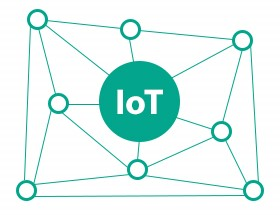
\includegraphics[scale=0.8]{img/part1/2.1}
    \caption{Internet of Things}
\end{figure}
